\documentclass[twocolumn,11pt]{article}
\setlength{\textheight}{9truein}
\setlength{\topmargin}{-0.9truein}
\setlength{\parindent}{0pt}
\setlength{\parskip}{10pt}
\setlength{\columnsep}{.4in}

\usepackage{amsmath,amsfonts,amssymb,amsthm,bm,caption,calc,ifthen,graphicx,url,hyperref}

\begin{document}
\pagestyle{plain}
\onecolumn
ASTP720 
\newline Homework 3
\newline Will Wainwright
\newline Repository: \href{https://github.com/wjwainwright/ASTP720}{https://github.com/wjwainwright/ASTP720}

\section*{Writeup}
Writing the ode library was pretty straightforward because we were given the iterable function forms in the notes. In order to make my methods work with simultaneous equations, I hard coded it to work for either one or two equations, given in the form of a list. For all three of my methods, I choose to append the initial conditions to the list of y-values and then appended $y_{i+1}$ based on the current $i$ value. I attempted to test each of my methods on a random function I came up with, but it proved to be pretty useless because I don't know the analytic solution to the differential equation. I compared the solutions from my ODE library to those obtained by Scipy's ODEint by using the simple pendulum example from Scipy's documentation. Figures 1-4 show that all three of my methods were effective in determining solutions to $\theta(t)$ and $\omega(t)$ that at least by eye are nearly identical to that of ODEint.

For the stiff ODE I choose a lambda value of 15. Upon plotting the results of my RK4 solver I found that the fit was terrible, but I also noticed that the plotted analytic solution started at $(0,1)$ and not $(0,0)$. I then changed the initial conditions that I gave my RK4 solver and fit the analytic solution perfectly. To my surprise, both Heun's method and the Euler method were also able to fit the analytic solution seemingly just as well as the RK4. The plots can be seen in figures 5-7.

Unfortunately, I was not able to finish parts 4 and 5. I wrote a hydro-static equilibrium function for a white dwarf to test my RK4 solver on, but after lots of time tinkering with it I only obtain a solution of an array of zeros for both differential equations. I feel bad that for two homeworks in a row now I have been able to write a library of methods but not been able to actually apply them to a real astronomy problem, but I would rather get this assignment in now as it is already several days late. 

\begin{figure}[!h]
	\centering
	\noindent
	\makebox[\textwidth]{
      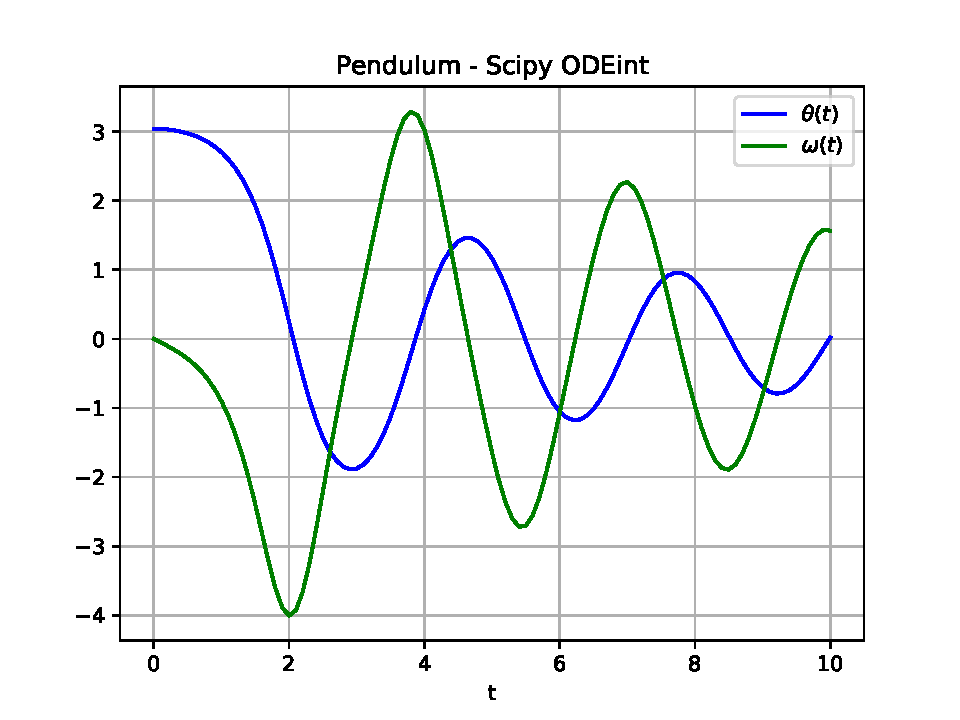
\includegraphics[width=4.5in]{odeint.pdf}}
      \caption{Plot of a simple pendulum solved using Scipy ODEint.}
\end{figure}

\begin{figure}[!h]
	\centering
	\noindent
	\makebox[\textwidth]{
      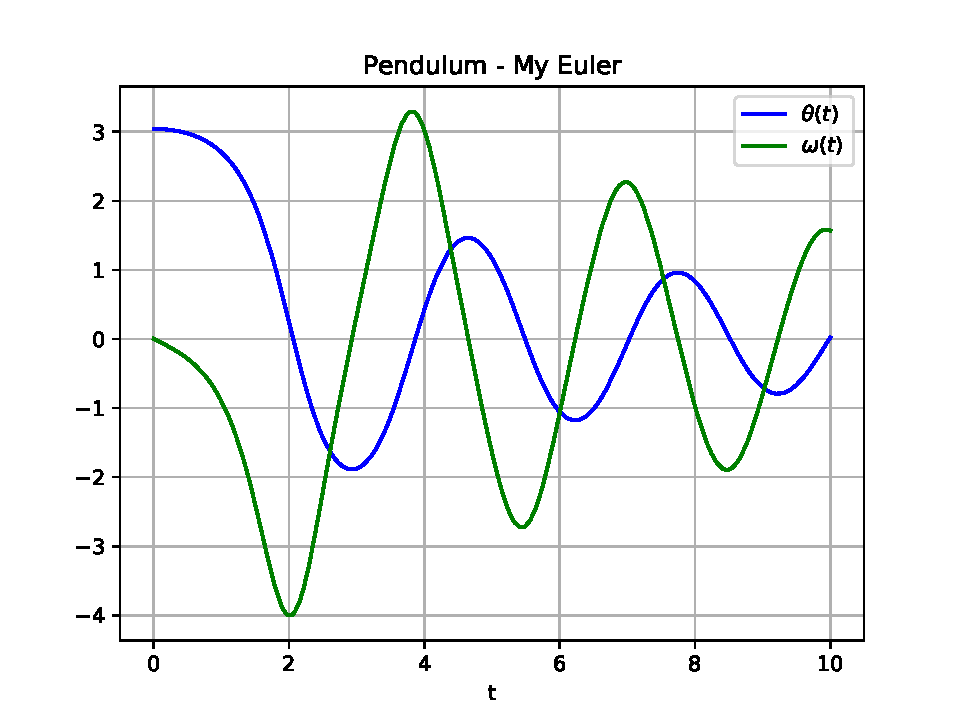
\includegraphics[width=4.5in]{euler.pdf}}
      \caption{Plot of a simple pendulum solved using my Euler method.}
\end{figure}

\begin{figure}[!h]
	\centering
	\noindent
	\makebox[\textwidth]{
      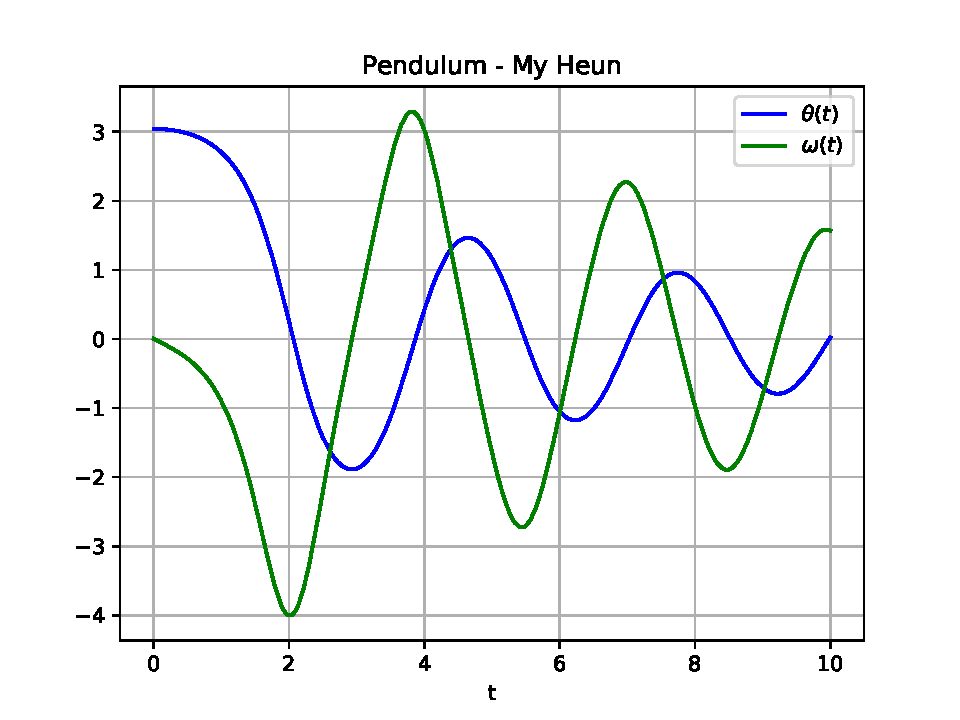
\includegraphics[width=4.5in]{heun.pdf}}
      \caption{Plot of a simple pendulum solved using my Heun's method.}
\end{figure}

\begin{figure}[!h]
	\centering
	\noindent
	\makebox[\textwidth]{
      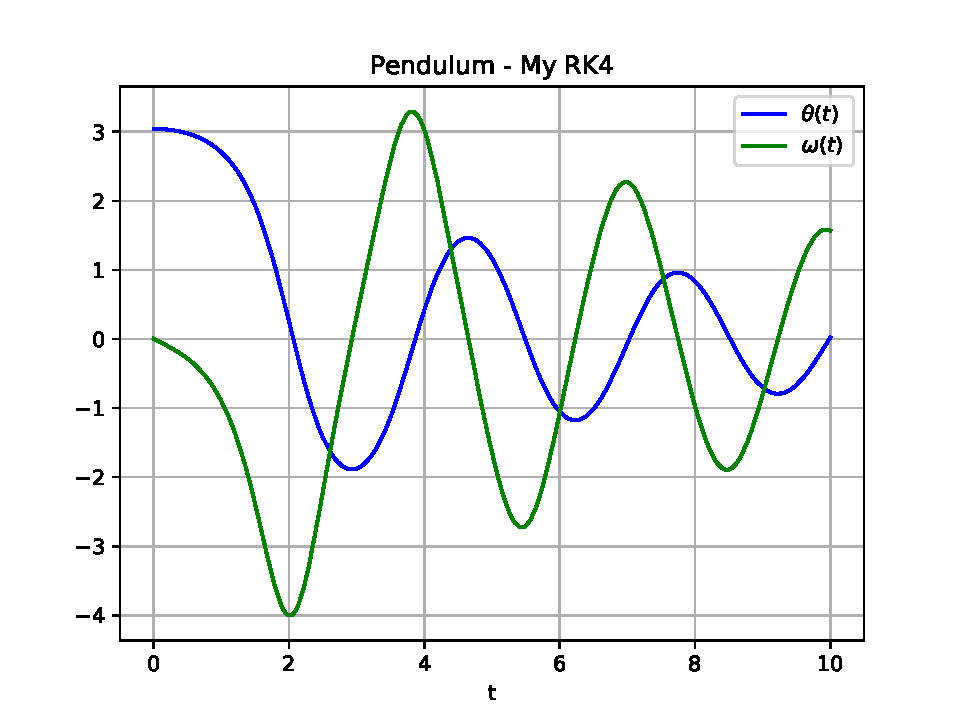
\includegraphics[width=4.5in]{rk4.pdf}}
      \caption{Plot of a simple pendulum solved using my RK4 method.}
\end{figure}

\begin{figure}[!h]
	\centering
	\noindent
	\makebox[\textwidth]{
      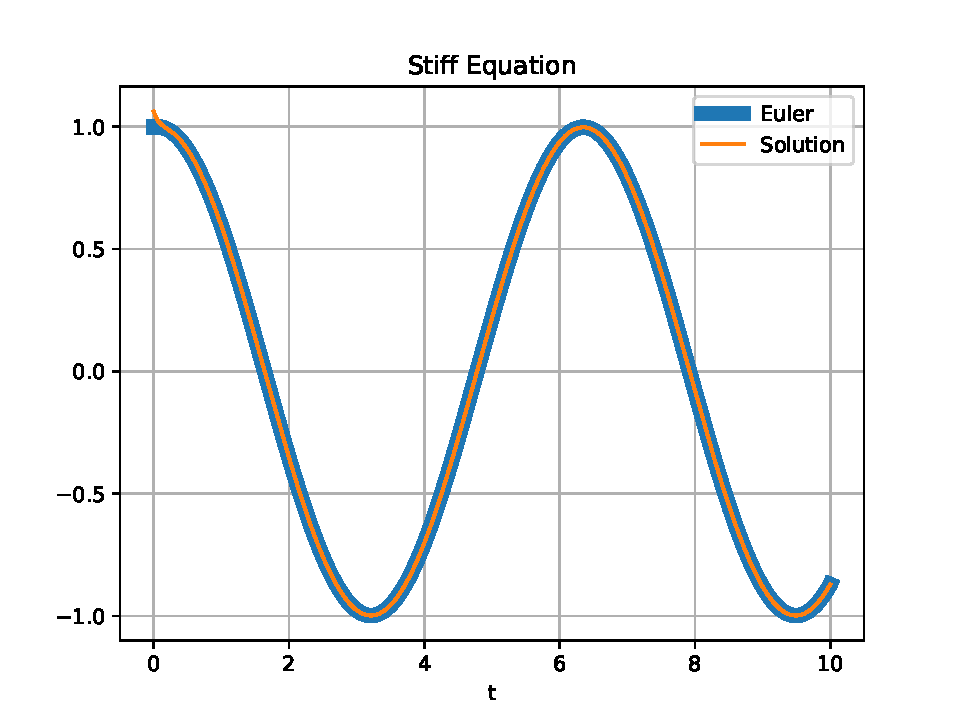
\includegraphics[width=4.5in]{stiff1.pdf}}
      \caption{Plot of a stiff function compared to its analytic solution. Solved using the Euler method.}
\end{figure}

\begin{figure}[!h]
	\centering
	\noindent
	\makebox[\textwidth]{
      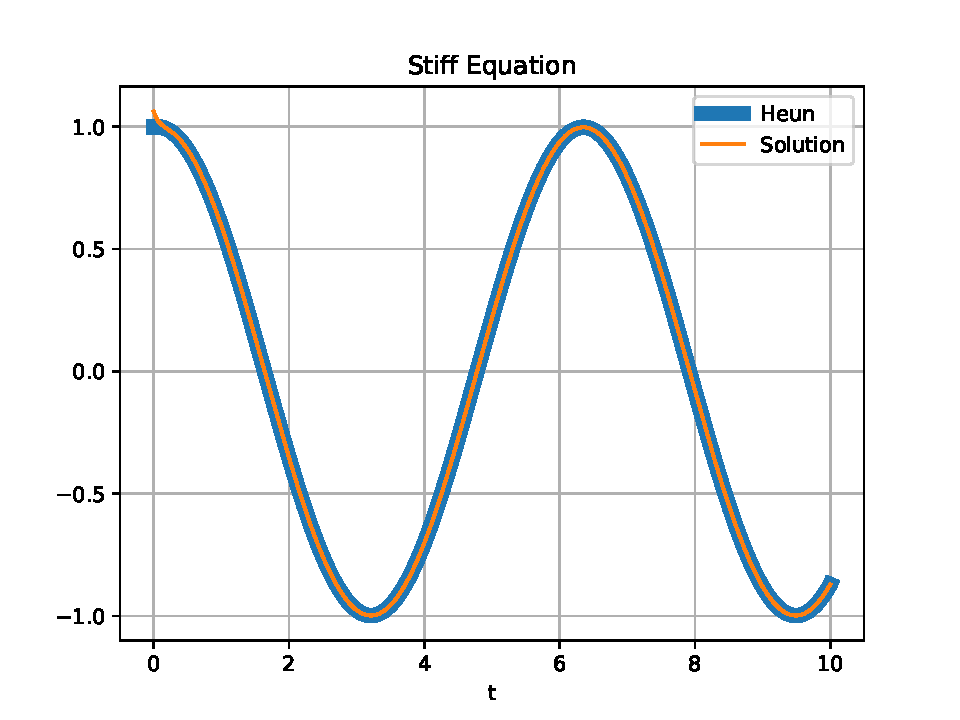
\includegraphics[width=4.5in]{stiff2.pdf}}
      \caption{Plot of a stiff function compared to its analytic solution. Solved using Heun's method.}
\end{figure}

\begin{figure}[!h]
	\centering
	\noindent
	\makebox[\textwidth]{
      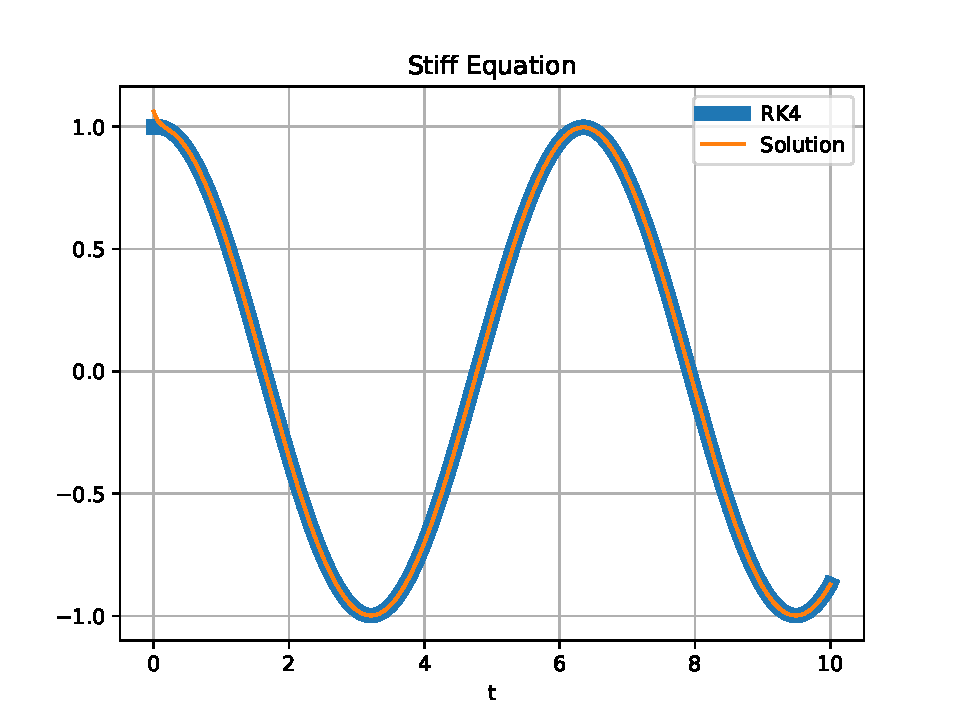
\includegraphics[width=4.5in]{stiff3.pdf}}
      \caption{Plot of a stiff function compared to its analytic solution. Solved using the RK4 method.}
\end{figure}

\end{document}